%iffalse
\let\negmedspace\undefined
\let\negthickspace\undefined
\documentclass[journal,12pt,onecolumn]{IEEEtran}
\usepackage{cite}
\usepackage{amsmath,amssymb,amsfonts,amsthm}
\usepackage{algorithmic}
\usepackage{graphicx}
\usepackage{textcomp}
\usepackage{xcolor}
\usepackage{txfonts}
\usepackage{listings}
\usepackage{enumitem}
\usepackage{mathtools}
\usepackage{pgfplots}
\usepackage{gensymb}
\usepackage{comment}
\usepackage[breaklinks=true]{hyperref}
\usepackage{tkz-euclide} 
\usepackage{listings}
\usepackage{gvv}                                        
%\def\inputGnumericTable{}                                 
\usepackage[latin1]{inputenc}                                
\usepackage{color}                                            
\usepackage{array}                                            
\usepackage{longtable}                                       
\usepackage{calc}                                             
\usepackage{multirow}                                         
\usepackage{hhline}                                           
\usepackage{ifthen}                                           
\usepackage{lscape}
\usepackage{tabularx}
\usepackage{array}
\usepackage{float}

\usepackage{enumitem}
\usepackage{xcolor}
%\usepackage{multicol}


\newtheorem{theorem}{Theorem}[section]
\newtheorem{problem}{Problem}
\newtheorem{proposition}{Proposition}[section]
\newtheorem{lemma}{Lemma}[section]
\newtheorem{corollary}[theorem]{Corollary}
\newtheorem{example}{Example}[section]
\newtheorem{definition}[problem]{Definition}
\newcommand{\BEQA}{\begin{eqnarray}}
\newcommand{\EEQA}{\end{eqnarray}}
\newcommand{\define}{\stackrel{\triangle}{=}}
\theoremstyle{remark}
\newtheorem{rem}{Remark}

\title{2009-PH-1-12}
\author{AI24BTECH11023 - Tarun Reddy Pakala}
\begin{document}
\bibliographystyle{IEEEtran}

\maketitle
\bigskip
\renewcommand{\thefigure}{\theenumi}
\renewcommand{\thetable}{\theenumi}
\begin{enumerate}
    \item The value of the contour integral, $\abs{\int_{C} \overrightarrow{r} \times d\overrightarrow{\theta} \, }$, for a circle $C$ of radius $r$ with center at origin is
    \begin{enumerate}
    \item $2\pi r$
    \item $r^2/2$
    \item $\pi r^2$
    \item $r$
    \end{enumerate}
    \item An electrostatic field $\overrightarrow{E}$ exists in a given region R. Choose the WRONG statement.
    \begin{enumerate}
    \item Circulation of $\overrightarrow{E}$ is zero
    \item $\overrightarrow{E}$ can always be expressed as the gradient of a scalar field
    \item The potential difference between any two arbitrary points in the region R is zero
    \item The work  done in a closed path lying entirely in R is zero
    \end{enumerate}
    \item The Lagrangian of a free particle in spherical polar co-ordinates is given by $L = \frac{1}{2} m \left( \dot{r}^2 + r^2 \dot{\theta}^2 + r^2 \dot{\phi}^2 \sin^2 \theta \right)$. The quantity that is conserved is
    \begin{enumerate}
    \item $\frac{\partial L}{\partial \dot{r}}$
    \item $\frac{\partial L}{\partial \dot{\theta}}$
    \item $\frac{\partial L}{\partial \dot{\phi}}$
    \item $\frac{\partial L}{\partial \dot{\phi}} + \dot{r} \dot{\theta}$
    \end{enumerate}
    \item A conducting loop $L$ of surface area $S$ is moving with a velocity $\overrightarrow{v}$ in a magnetic field $\overrightarrow{B}(\overrightarrow{r},t)$=$\overrightarrow{B_0}t^2$, $B_o$ is a positive constant of suitable dimensions. The emf induced, $V_{emf}$, in the loop is given by
    \begin{enumerate}
        \item -$\int_S \frac{\partial \overrightarrow{B}}{\partial t} \cdot d\overrightarrow{S}$
        \item $\oint_L (\overrightarrow{v} \times \overrightarrow{B}) \cdot d\overrightarrow{L}$
        \item -$\int_S \frac{\partial \overrightarrow{B}}{\partial t} \cdot d\overrightarrow{S}$-$\oint_L (\overrightarrow{v} \times \overrightarrow{B}) \cdot d\overrightarrow{L}$
        \item -$\int_S \frac{\partial \overrightarrow{B}}{\partial t} \cdot d\overrightarrow{S}$+$\oint_L (\overrightarrow{v} \times \overrightarrow{B}) \cdot d\overrightarrow{L}$
    \end{enumerate}
    \item The eigenvalues of the matrix $A= 
\begin{bmatrix}
0 & i \\
i & 0
\end{bmatrix}
$ are
    \begin{enumerate}
    \item real and distinct
    \item complex and distinct
    \item complex and coinciding
    \item real and coinciding
    \end{enumerate}
    \item $\sigma_i(i=1, 2, 3)$ represent the Pauli spin matrices. Which one of the following is NOT true ?
    \begin{enumerate}
        \item $\sigma_i \sigma_j$+$\sigma_j \sigma_i$=2$\delta_{ij}$
        \item $Tr(\sigma_i)=0$
        \item The eigenvalues of $\sigma_i$ are $\pm1$
        \item det($\sigma_i$)=1
    \end{enumerate}
    \item Which one of the functions given below represents the bound state eigenfunction of the operator $ - \frac{d^2}{dx^2} $ in the region, $0 \leq x < \infty$ with the eigenvalue -4 ? 
    \begin{enumerate}
    \item $A_o e^{2x}$
    \item $A_o \cosh{2x}$
    \item $A_o e^{-2x}$
    \item $A_o \sinh{2x}$
    \end{enumerate}
    \item Pick the WRONG statement.
    \begin{enumerate}
        \item The nuclear force is independent of electric charge
        \item The Yukawa potential is proportional to $r^{-1} \exp\left(\frac{mc}{\hbar} r\right)$, where $r$ is the separation between two nucleons
        \item The range of nuclear force is order of $10^{-15}m-10^{-14}m$
        \item The nucleons interact among each other by the exchange of mesons
    \end{enumerate}
    \item If $p$ and $q$ are the position and momentum variables, which one of the following is NOT a canonical transformation ?
    \begin{enumerate}
        \item $Q=\alpha q$ and $P= \frac{1}{\alpha}p$, for $\alpha \neq 0$
        \item $Q=\alpha q+\beta p$ and $P=\beta q+\alpha p$ for $\alpha,\beta$ real and $\alpha^2-\beta^2=1$
        \item $Q=p$ and $P=q$
        \item $Q=p$ and $P=-q$
    \end{enumerate}
    \item The Common Mode Rejection Ratio (CMRR) of a differential amplifier using an operational amplifier is 100 dB. The output voltage for a differential input of 200 $\mu$V is 2 V. The common mode gain is
    \begin{enumerate}
        \item 10
        \item 0.1
        \item 30 dB
        \item 10 dB
    \end{enumerate}
    \item In an insulating solid which one of the following physical phenomena is a consequence of Pauli's exclusion principle ?
    \begin{enumerate}
        \item Ionic conductivity
        \item Ferromagnetism
        \item Paramagnetism
        \item Ferroelectricity
    \end{enumerate}
    \item Which one of the following curves gives the solution of the differential equation $k_1 \frac{dx}{dt} + k_2 x = k_3$, where $k_1,k_2$ and $k_3$ are positive constants with initial conditions $x=0$ at $t=0$ ?
    \begin{enumerate}
        \item 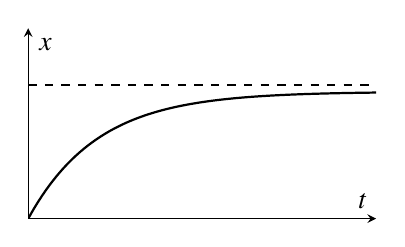
\begin{tikzpicture}
    \begin{axis}[
        axis lines=middle, 
        xlabel={$t$}, 
        ylabel={$x$},
        xmin=0, xmax=5, ymin=0, ymax=1.5,
        xtick=\empty, ytick=\empty,
        domain=0:5,
        samples=100,
        width=6cm,
        height=4cm,
    ]
    \addplot[smooth, thick] {1 - exp(-x)}; 
    \addplot[dashed, thick] coordinates {(0,1.05) (5,1.05)}; 
    \end{axis}
\end{tikzpicture}
        \item \begin{tikzpicture}
    \begin{axis}[
        axis lines=middle, 
        xlabel={$t$}, 
        ylabel={$x$},
        xmin=0, xmax=5, ymin=0, ymax=8.6, 
        xtick=\empty, ytick=\empty,
        domain=0:5,
        samples=100,
        width=6cm,
        height=4cm,
    ]
    \addplot[smooth, thick] {x^2}; 
    \addplot[dashed, thick] coordinates {(3,0) (3,9)}; 
    \end{axis}
\end{tikzpicture}
        \item 
        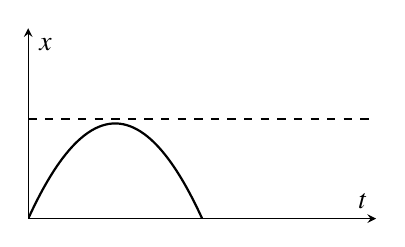
\begin{tikzpicture}
    \begin{axis}[
        axis lines=middle, 
        xlabel={$t$}, 
        ylabel={$x$},
        xmin=0, xmax=4, ymin=0, ymax=2,
        xtick=\empty, ytick=\empty,
        domain=0:4,
        samples=100,
        width=6cm,
        height=4cm,
    ]
    % Function: y = x(2 - x)
    \addplot[smooth, thick] {x * (2 - x)};
    
    % Calculate the maximum y-coordinate
    \pgfmathsetmacro{\maxY}{1}  % Maximum occurs at x=1
    \pgfmathsetmacro{\offset}{0.05}  % Small offset to position dashed line above the maxY
    
    % Horizontal dashed line just above the maximum point
    \addplot[dashed, thick] coordinates {(0, \maxY + \offset) (4, \maxY + \offset)}; 

    \end{axis}
\end{tikzpicture}

        \item 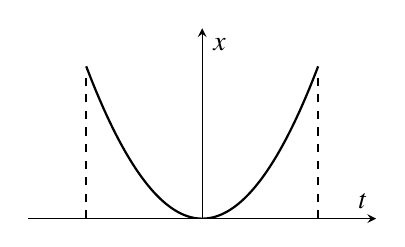
\begin{tikzpicture}
    \begin{axis}[
        axis lines=middle, 
        xlabel={$t$}, 
        ylabel={$x$},
        xmin=-3, xmax=3, ymin=0, ymax=5,
        xtick=\empty, ytick=\empty,
        domain=-2:2, 
        samples=100,
        width=6cm,
        height=4cm
    ]
    \addplot[smooth, thick] {x^2}; 
    \addplot[dashed, thick] coordinates {(-2,0) (-2,3.7)};
    \addplot[dashed, thick] coordinates {(2,0) (2,3.7)};
    \end{axis}
\end{tikzpicture}
    \end{enumerate}
\end{enumerate}
\end{document}
